\section{Linear separability}


\begin{frame}\frametitle{\secname}

\underline{Setting}:\\

\begin{equation*}
\Big\{ \left(\vec x^{(\alpha)}, y^{(\alpha)}_{\mathrm{T}} \right) \Big\}\,,\quad \alpha = 1,\ldots,p
\end{equation*}

\begin{itemize}
\item $p$ points
\item $N$ dimensions $\vec x \in \R^N$
\item binary assignment: $y_T \in \{-1,1\}$
\end{itemize}

\pause

\underline{Model}:\\

Linear neuron with $N$ weights and a bias ($N+1$ degrees of freedom).

\pause

\underline{Task}:\\

Find the total number of binary assignments that are linearly separable.

\end{frame}

\begin{frame}\frametitle{Find the total number of affinely separable assignments}

\begin{enumerate}
\item Place $p$ points in $N$ dimensions, any way you like as long as they're not collinear.
\item Assign all possible labels to the points.
\end{enumerate}

Example with 4 points in 2D:

\mode<presentation>{
\textbf{see blackboard...}
}

\question{How many assignment configurations are there?}\\


\question{How many of them can be separated by a connectionist neuron?}

\end{frame}

\begin{frame}
		\begin{figure}[h]
			\centering
			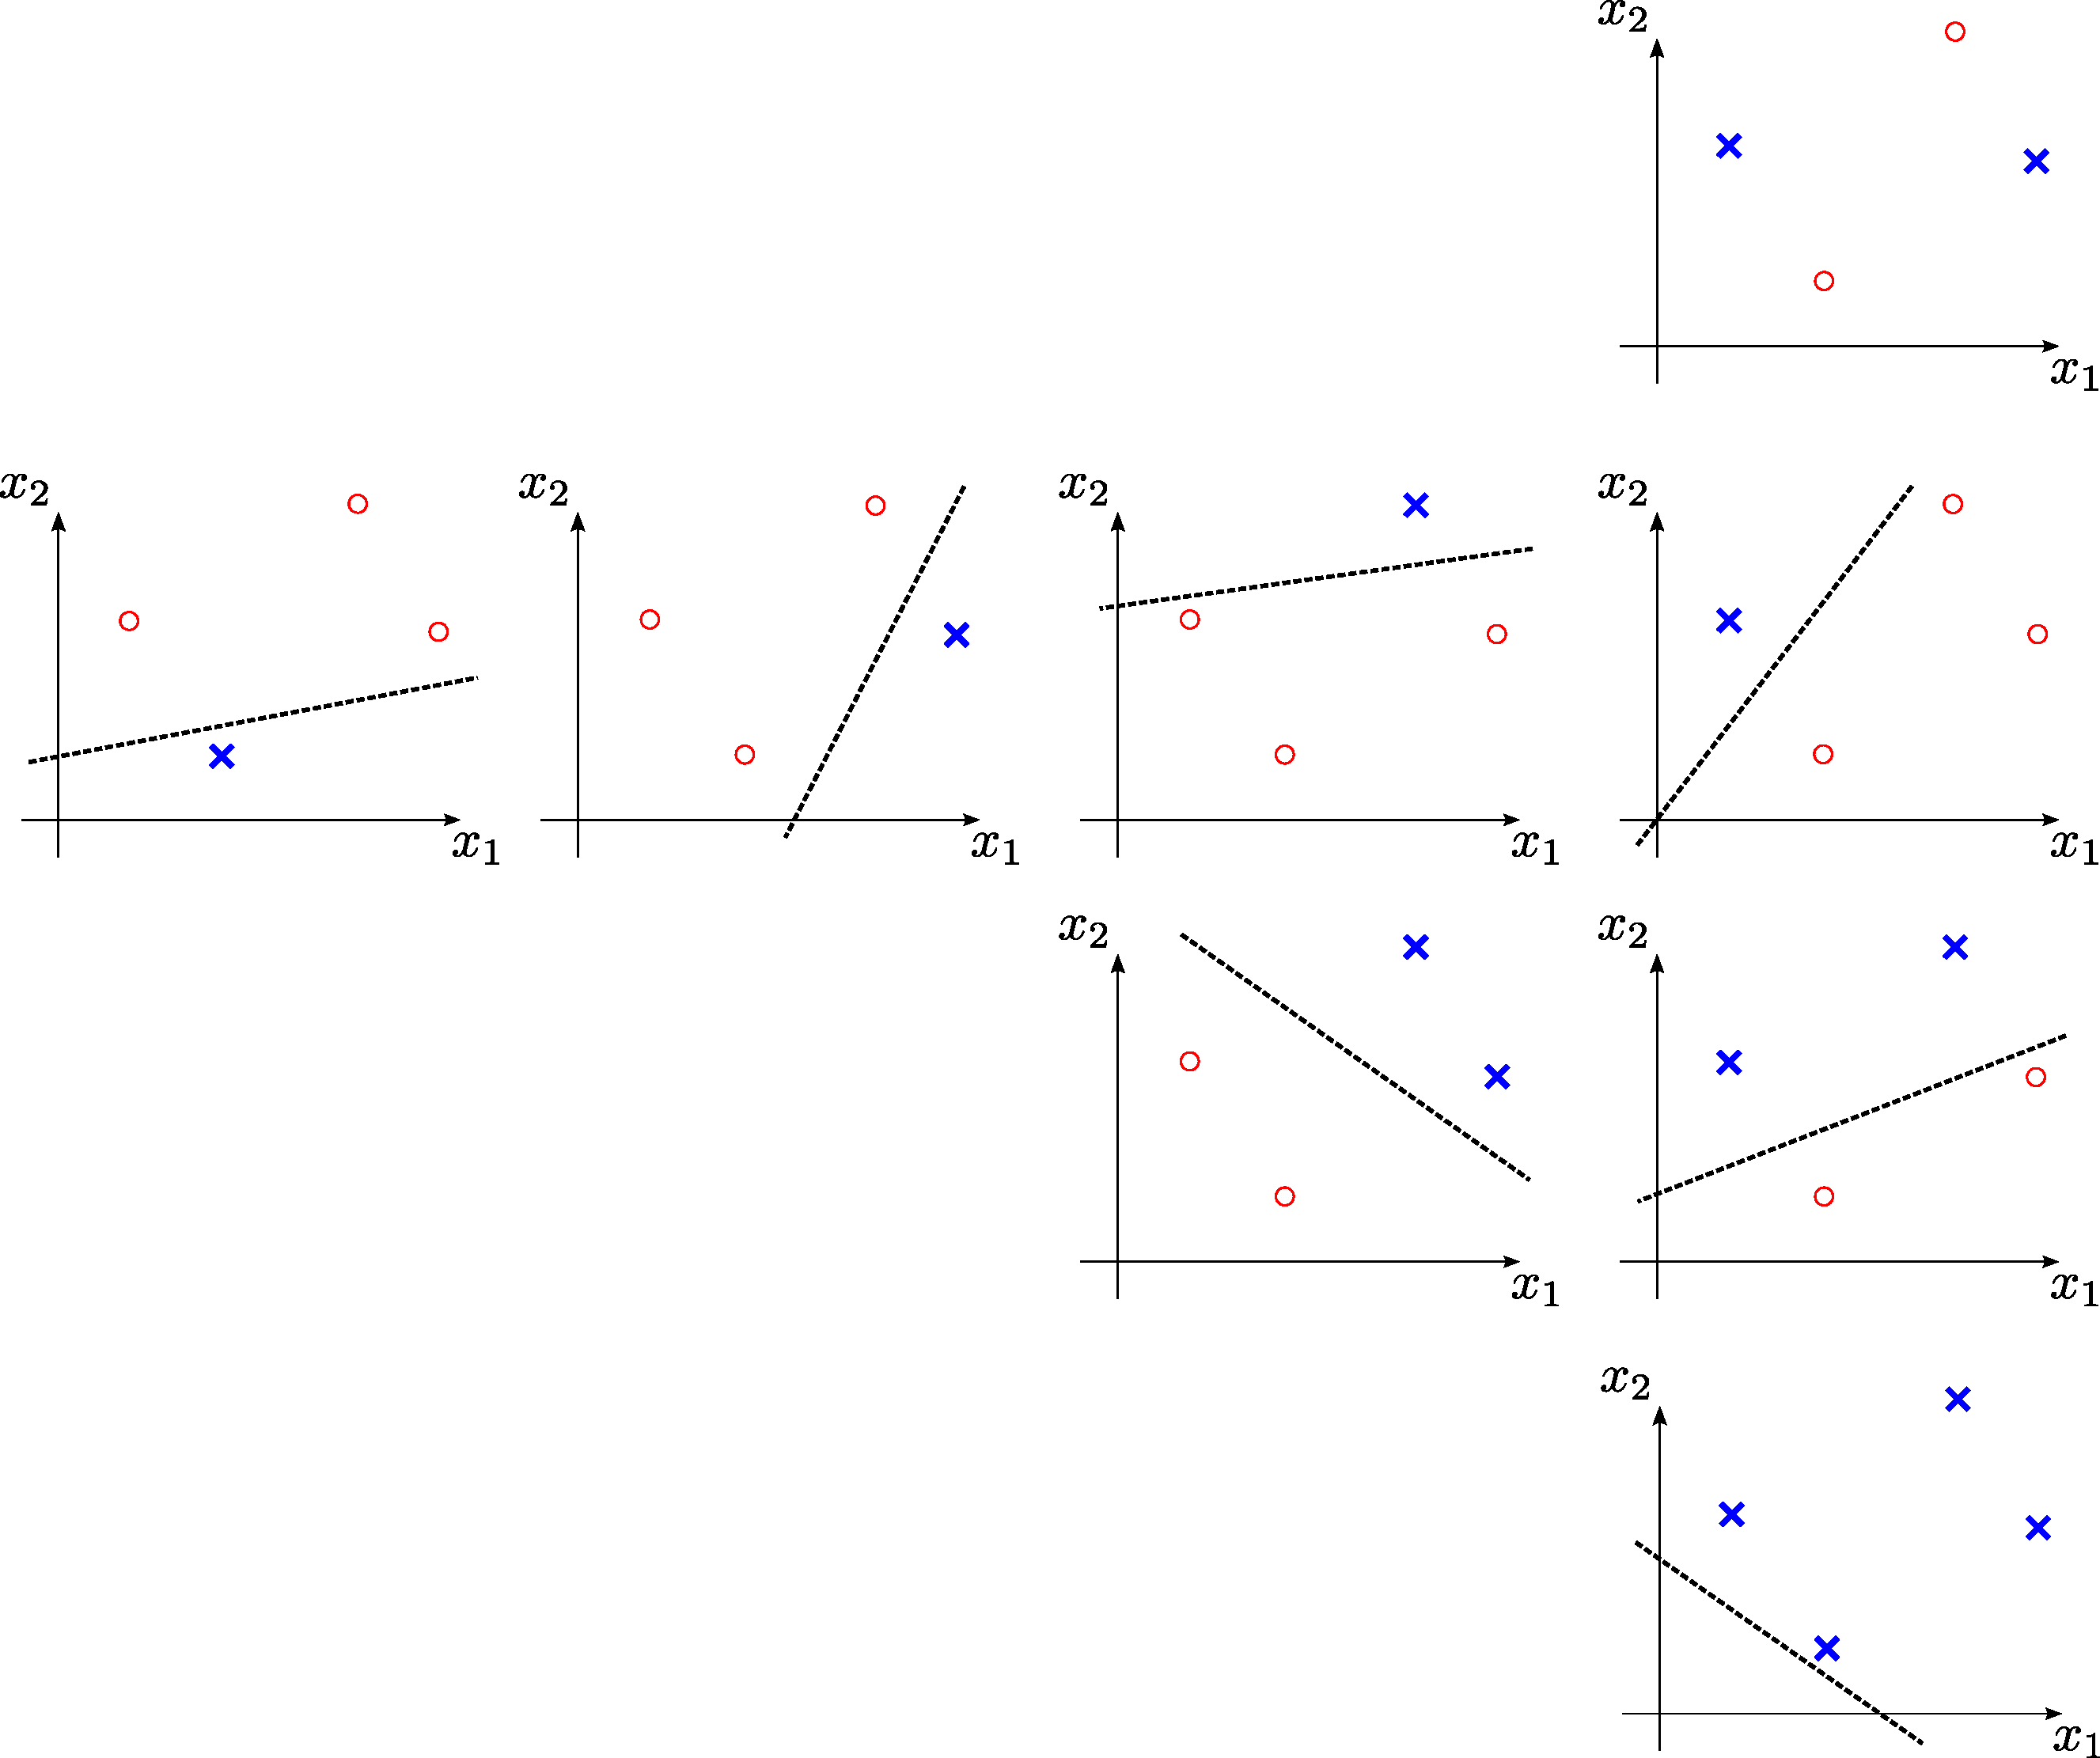
\includegraphics[width=0.85\textwidth]{img/linearly_sep}
            \mode<article>{
			\caption{Classifying 4 points in 2D. Multiply by 2 (reverse classification) to get all possible $2^4 = 16$ configurations. 2 of those configurations, the XOR- (top-right) and XNOR-like configurations are not linearly separable.}
            }
		\end{figure}
\end{frame}

\begin{frame}\frametitle{Calculate the number of configurations that are linearly separable}

Calculate the number of linearly separable assignments:

\begin{equation}
	\tilde C_{(p,N)} := 2 \sum_{k=0}^{N} 
	\underbrace{
	\left( \begin{array}{c}
	p-1\\
	k
	\end{array}\right)
	}_{\substack{\text{Binomial}\\ \text{coefficient}}}
\end{equation}

The Binomial coefficient\footnote{
See \href{https://en.wikipedia.org/wiki/Pascal\%27s_triangle}{Pascal's triangle} for a fun way on how to manually compute the coefficient.
} 
(``$n$ choose $k$'') 
is defined as:

\begin{equation}
\left(n \atop k \right) = \frac{n!}{k! (n-k)!}
\end{equation}

for $n,k \in \N_0$ with $n \ge k \ge 0$

\end{frame}

%\begin{frame}\frametitle{The Binomial coefficient}
\mode<article>{
The Binomial coefficient represents the coefficient associated with the $y^k$ term in the polynomial expansion $(1+y)^n$.

Consider the following example\footnote{
The example is taken from the Wikipedia article on \href{https://en.wikipedia.org/wiki/Binomial_coefficient}{Binomial coefficient}
} of using polynomial expansion for calculating the fourth power of $(1+y)$:

\begin{align}
(1+y)^4 &= 
\left({4 \atop 0}\right) y^0 +
\left({4 \atop 1}\right) y^1 +
{\color{blue}\left({4 \atop 2}\right) y^2} +
\left({4 \atop 3}\right) y^3 +
\left({4 \atop 4}\right) y^4\\
&= 1 + 4y + {\color{blue}6y^2} + 4y^3 + y^4
\label{eq:polyexpansion}
\end{align}

The binomial coefficient $\left({4 \atop 2}\right) = \frac{4!}{2!(4-2)!} = 6$. ${\color{blue}6}$ matches the coefficient in front of the ${\color{blue}y^2}$ term in the expansion\notesonly{ in \eqref{eq:polyexpansion}}.
}
%\end{frame}

\begin{frame}\frametitle{Calculating the number of separable configurations?}

\begin{equation*}
	\tilde C_{(p,N)} := 2 \sum_{k=0}^{N} \left( \begin{array}{c}
	p-1\\
	k
	\end{array}\right)
	\label{eq:cwithbias}
\end{equation*}

Using our example with $p=4$ and $N=2$:
\begin{align}
	\tilde C_{(4,2)} &= 2 \sum_{k=0}^{2} \left( \begin{array}{c}
	4-1\\
	k
	\end{array}\right)\\
	&= 2 \,
	\bigg\lbrack
	%\underbrace{
	\left({4-1 \atop {\color{black}0}}\right)
	%}_{\substack{\text{all positive}\\ \text{{\color{red}none} negative}}}
	+
	%\underbrace{
	\left({4-1 \atop {\color{black}1}}\right)
	%}_{\substack{\text{{\color{red}1} out of p}\\ \text{negative}}}
	+
	%\underbrace{
	\left({4-1 \atop {\color{black}2}}\right)
	%}_{\substack{\text{{\color{red}2} out of p}\\ \text{negative}}}
	\bigg\rbrack\\
	&= 2 \, \Big\lbrack
	1 + 3 + 3
	\Big\rbrack\\
	&= 14
\end{align}


\end{frame}

\begin{frame}

\mode<presentation>{

\begin{equation*}
	\tilde C_{(p,N)} := 2 \sum_{k=0}^{N} \left( \begin{array}{c}
	p-1\\
	k
	\end{array}\right)
\end{equation*}
}

\textbf{But} this looks slightly different from what is in the lecture. In the lecture it looked like this:

\begin{equation}
	C_{(p,N)} := 2 \sum_{k=0}^{N-1} \left( \begin{array}{c}
	p-1\\
	k
	\end{array}\right)
	\label{eq:cnobias}
\end{equation}

\question{Why does the sum for $\tilde C_{(p,N)}$ run to $N$ instead of $N-1$?}\\

\mode<article>{
-The difference between $\tilde C_{(p,N)}$ from \eqref{eq:cwithbias} and $C_{(p,N)}$ from \eqref{eq:cnobias} look different is due to the fact that $\tilde C_{(p,N)}$ computes the sum for $k=1,\ldots,N$ instead of stopping at $N$ is that sum iterates over the degrees of freedom. 
Choosing a connectionist neuron to the separation involves $N+1$ degrees of freedom because we add the bias term (the ability to translate the hyperplane).
Therefore, the reason is the model choice and assuming that $C_{(p,N)}$ counts separability around the origin without the ability to shift the hyperplane.

-An alternative explanation to the difference between $\tilde C_{(p,N)}$ and $C_{(p,N)}$ is how to interpret $N$. The definition of $C_{(p,N)}$ treats $N$ as the parameters of the hyperplane. Therefore the bias is implicit.
If we assume that $N$ is the number of components in $\vec x$ and we need to prepend a bias term to it, we compute the number of separable configurations using $\tilde C_{(p,N)}$. 
It is important to understand that $\tilde C_{(p,N)}$ and $C_{(p,N)}$ effectively yield the same result when we feed each the appropriate arguments.
}
\end{frame}

\begin{frame}
Recursive formula for the binomial coefficient:
\begin{equation}
			\left( \begin{array}{c}
			n\\
			k
			\end{array}\right)+
			\left( \begin{array}{c}
			n\\
			k-1
			\end{array}\right)=
			\left( \begin{array}{c}
			n+1\\
			k
			\end{array}\right)
\end{equation}

Use the the recursive formula for the binomial coefficient to show that:

\begin{equation}
\tilde C_{(p,N)}+\tilde C_{(p,N-1)}=\tilde C_{(p+1,N)}
\label{eq:c_relation}
\end{equation}

The relevance of \notesonly{\eqref{eq:c_relation}}\slidesonly{ this} relationship becomes apparent when attempting to derive the VC dimension\notesonly{ (introduced in \sectionref{seq:dvc})} of a connectionist neuron.

\end{frame}

\begin{frame}
\mode<presentation>{
\only<1,2>{Show that}
\vspace{-5mm}
}

{
\begin{align}
\only<1,2>{
	\tilde C_{(p,N)} 
	\qquad + \quad \tilde C_{(p,N-1)} \;\;\quad
    &= \slidesonly{\qquad} \tilde C_{(p+1,N)}\qquad\\
    \notesonly{
	\intertext{Plugging in \eqref{eq:cwithbias} for each:}
	}
}
\only<1-4>{
    2 \sum_{k=0}^{N} \left(\kern-1ex \begin{array}{c}
	p-1\\
	k
	\end{array} \kern-1ex \right)
    +
    2 \sum_{k=0}^{N-1} \left(\kern-1ex \begin{array}{c}
	p-1\\
	k
	\end{array} \kern-1ex \right)
    &= 
    2 \sum_{k=0}^{N} \left(\kern-1ex \begin{array}{c}
	p+1-1\\
	k
	\end{array} \kern-1ex \right)\only<4->{\slidesonly{\\[-20mm]}
}
}
\only<2-4>{
	\intertext{Simplify the LHS by modifying the sums \notesonly{such that}\slidesonly{s.t.} they share the same limits.}
}
\only<2-5>{
	{\color{magenta}
    2 \left(\kern-1ex \begin{array}{c}
	p-1\\
	0
	\end{array}\kern-1ex\right)}
    +
    2 \sum_{k={\color{magenta}\cancel{0}1}}^{N} \left(\kern-1ex \begin{array}{c}
	p-1\\
	k
	\end{array} \kern-1ex \right)
    +
    2 \sum_{k=0}^{N{\only<3,4>{\color{red}}-1}} \left(\kern-1ex \begin{array}{c}
	p-1\\
	k
	\end{array}\kern-1ex\right)
    &= 
    2 \sum_{k=0}^{N} \left(\begin{array}{c}
	p\\k
	\end{array}\right)\\
}
\only<3-5>{
	{\color{magenta}
    2 \left(\kern-1ex \begin{array}{c}
	p-1\\ 0
	\end{array} \kern-1ex \right)}
    + 2~
    {\color{blue}
    \sum_{k=1}^{N}
    }\left(\kern-1ex \begin{array}{c}
	p-1\\ k
	\end{array} \kern-1ex \right)
    + 2~
    {\color{blue}
    \sum_{k=1}^{N}
    } \left(\kern-1ex \begin{array}{c}
	p-1\\ k{\color{red}-1}
	\end{array} \kern-1ex \right)
    &=\\
    %2 \sum_{k=0}^{N} \left( \begin{array}{c}
	%p\\ k
	%\end{array}\right)
	%\\
}
\only<4-5>{
	{\color{magenta}
    2 \left(\kern-1ex \begin{array}{c}
	p-1\\ 0
	\end{array} \kern-1ex \right)}
    + 2~
    {\color{blue}
    \sum_{k=1}^{N}
    }
    \bigg \lbrack \underbrace{
    \left(
    \begin{array}{c}
	p-1\\ k
	\end{array}\right)
    +\left(
    \begin{array}{c} 
	p-1\\ k-1
	\end{array}\right)
    }_{=\left(
    \begin{array}{c} 
	p\\ k
	\end{array}\right)\text{ (using the recursive property)}}
    \bigg 
    \rbrack
    &=\\
}
\only<5,6>{
    {\color{magenta}2} \underbrace{
		{\color{magenta}
		\left(\kern-1ex \begin{array}{c}
		p-1\\ 0
		\end{array} \kern-1ex \right)}
	}_{=1=\left( \begin{array}{c}
	p\\ 0
	\end{array}\right)}
    +
    2~{\color{blue}\sum_{k=1}^{N}}\left( \begin{array}{c}
	p\\ k
	\end{array}\right)
    &= 2 \sum_{k=0}^{N}
    \left( \begin{array}{c}
	p\\ k
	\end{array}\right)\\
\intertext{$\left({p \atop 0}\right)$ can now be \textcolor{red}{absorbed} into the sum.}
2 \sum_{k={\color{red}0}}^{N}
    \left( \begin{array}{c}
	p\\ k
	\end{array}\right)
    &=
2 \sum_{k=0}^{N}
    \left( \begin{array}{c}
	p\\ k
	\end{array}\right)
	}
\end{align}
}
\mode<presentation>{
\only<6>{
\begin{equation*}
\tilde C_{(p,N)}+\tilde C_{(p,N-1)}=\tilde C_{(p+1,N)}
\end{equation*}
}
}

\end{frame}
